\documentclass[12pt]{article}

\pagestyle{empty}
\setlength{\topmargin}{0in}
\setlength{\headheight}{0in}
\setlength{\topsep}{0in}
\setlength{\textheight}{9in}
\setlength{\oddsidemargin}{0in}
\setlength{\evensidemargin}{0in}
\setlength{\textwidth}{6.5in}

\usepackage{palatino,graphics,amsmath,amssymb,enumitem}

\newcommand{\ds}{\displaystyle}
\newcommand{\vs}[1]{\vspace{#1in}}
\renewcommand{\vss}[1]{\vspace*{#1in}}
\newcommand{\bvec}{{\mathbf b}}
\newcommand{\cvec}{{\mathbf c}}
\newcommand{\dvec}{{\mathbf d}}
\newcommand{\evec}{{\mathbf e}}
\newcommand{\fvec}{{\mathbf f}}
\newcommand{\qvec}{{\mathbf q}}
\newcommand{\uvec}{{\mathbf u}}
\newcommand{\vvec}{{\mathbf v}}
\newcommand{\wvec}{{\mathbf w}}
\newcommand{\xvec}{{\mathbf x}}
\newcommand{\yvec}{{\mathbf y}}
\newcommand{\zvec}{{\mathbf y}}
\newcommand{\zerovec}{{\mathbf 0}}
\newcommand{\real}{{\mathbb R}}
\newcommand{\twovec}[2]{\left[\begin{array}{r}#1 \\ #2
    \end{array}\right]}
\newcommand{\ctwovec}[2]{\left[\begin{array}{c}#1 \\ #2
   \end{array}\right]}
\newcommand{\threevec}[3]{\left[\begin{array}{r}#1 \\ #2 \\ #3
  \end{array}\right]}
\newcommand{\cthreevec}[3]{\left[\begin{array}{c}#1 \\ #2 \\ #3
    \end{array}\right]}
\newcommand{\fourvec}[4]{\left[\begin{array}{r}#1 \\ #2 \\ #3 \\ #4
    \end{array}\right]}
\newcommand{\cfourvec}[4]{\left[\begin{array}{c}#1 \\ #2 \\ #3 \\ #4
    \end{array}\right]}
\newcommand{\mattwo}[4]{\left[\begin{array}{rr}#1 & #2 \\ #3 & #4 \\ \end{array}\right]}
\renewcommand{\span}[1]{\text{Span}\{#1\}}
\newcommand{\bcal}{{\cal B}}
\newcommand{\ccal}{{\cal C}}
\newcommand{\scal}{{\cal S}}
\newcommand{\wcal}{{\cal W}}
\newcommand{\ecal}{{\cal E}}
\newcommand{\coords}[2]{\left\{#1\right\}_{#2}}
\newcommand{\gray}[1]{\color{gray}{#1}}
\newcommand{\lgray}[1]{\color{lightgray}{#1}}
\newcommand{\rank}{\text{rank}}
\newcommand{\col}{\text{Col}}
\newcommand{\nul}{\text{Nul}}

\begin{document}

\noindent
{\bf Mathematics 227} \\ 
{\bf Markov chains}

\begin{enumerate}
\item Consider the stochastic matrix
  $A =
  \left[
    \begin{array}{cc}
      0.8 & 0.1 \\
      0.2 & 0.9 \\
    \end{array}
  \right]
  $.  Is this a positive matrix?

  \vs{1}
  Find the unique steady-state vector $\qvec$.

  \vs{1}
  What does the Perron-Froebenius theorem say about the convergence of
  a Markov chain beginning with some initial state vector $\xvec_0$?

  \vs{1}
  Consider the initial state vector $\xvec_0 = \twovec10$ and describe
  what happens when you
  generate 20 terms in the Markov chain using the following code after
  defining {\tt A} and {\tt x}:
\begin{verbatim}
for i in range(20):
    x = A*x
    print x
\end{verbatim}

  \vs{1}
  What happens to the Markov chain when you begin with the initial
  state vector 
  $\xvec_0=\twovec01$?

  \vs{1}
\item Consider the stochastic matrix
  $A =
  \left[
    \begin{array}{ccc}
      0 & 0 & 1 \\
      1 & 0 & 0 \\
      0 & 1 & 0 \\
    \end{array}
  \right]
  $.
  Look at a few powers of $A$ and determine whether $A$ is a positive
  matrix.

  \vs{1}
  What happens when you create a Markov chain beginning with the
  initial state vector $\threevec100$?

  \vs{1}
  Does the Perron-Frobenius theorem apply in this case?

  \vs{1}
\item Suppose that you live in a country having three political
  parties $P$, $Q$, and $R$.  We will use $P_k$, $Q_k$ and $R_k$ to
  denote the percentage of voters voting for each party in election
  $k$.  The state vector for an election is
  $\xvec_k = \threevec{P_k}{Q_k}{R_k}$.
  
  Voters will change parties from one election to the next as shown in
  the figure.

  \begin{center}
    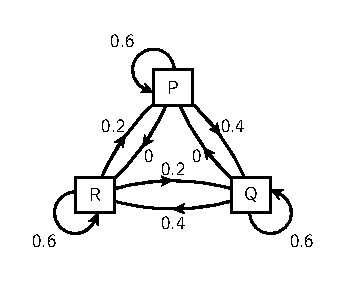
\includegraphics{stoch-parties.eps}
  \end{center}

  \newpage
  Find the matrix $A$ such that $\xvec_{k+1}=A\xvec_k$.

  \vs{1}
  Explain why $A$ is a stochastic matrix.

  \vs{1}
  Suppose that initially 40\% of voters vote for party $P$, 30\% vote
  for party $Q$, and 30\% of voters vote for party $R$.  What is
  $\xvec_0$ and why should it be a probability vector?

  \vs{1}
  Does the Perron-Frobenius theorem apply?  If so, what does it imply?

  \vs{1}
  Find the unique steady-state vector $\qvec$.

  \vs{1}
  What happens to the Markov chain after a very long time?

  \vs{1}
  Generate 20 terms in a Markov chain to confirm your prediction.

  
  



\end{enumerate}


\end{document}
